% %%%%%%%%%%%%%%%%%%%%%%%%%% Figure 1 Oversiktskart %%%%%%%%%%%%%%%%%%%%%%%%%%%%
\begin{figure}[t]
 \setlength{\unitlength}{1.0cm}
 \begin{center}
  \begin{pspicture}(0,0)(15,9)
% Include graphs
   \rput[bl](0,0){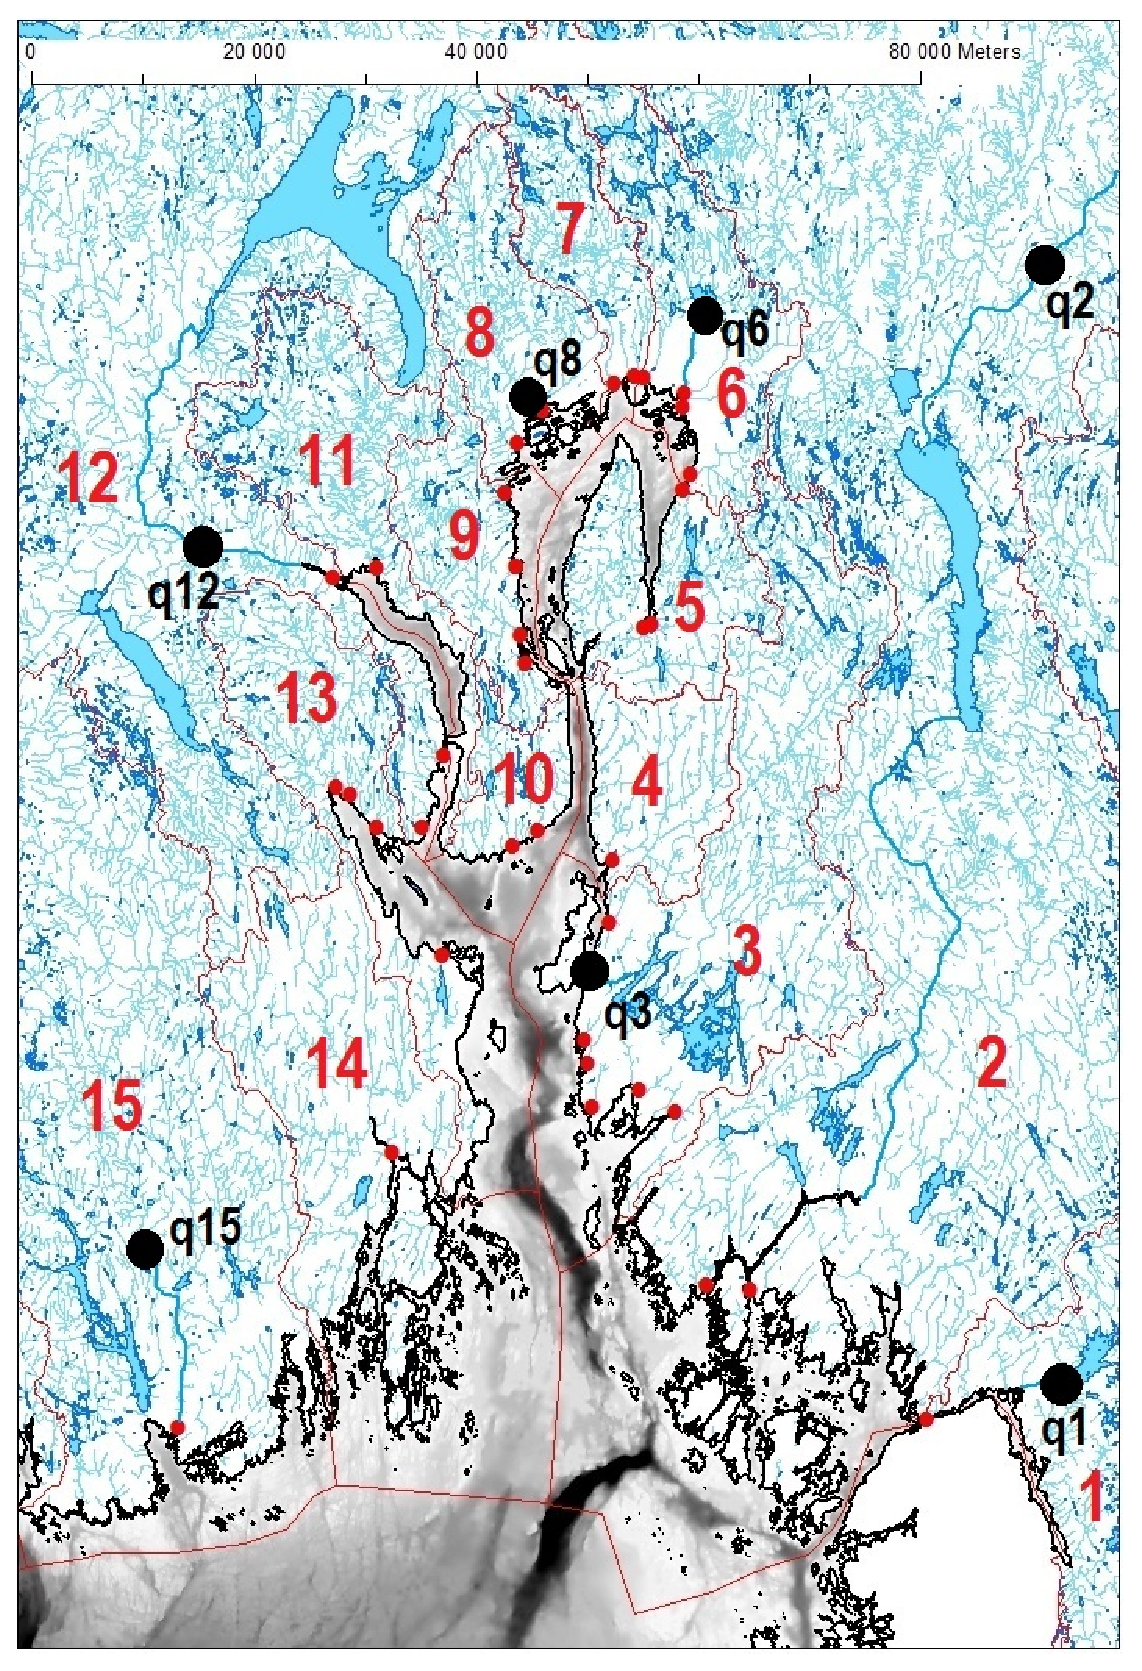
\includegraphics[height=9cm]{Elver_Oslofjorden_v4}}
   \rput[br](15,0){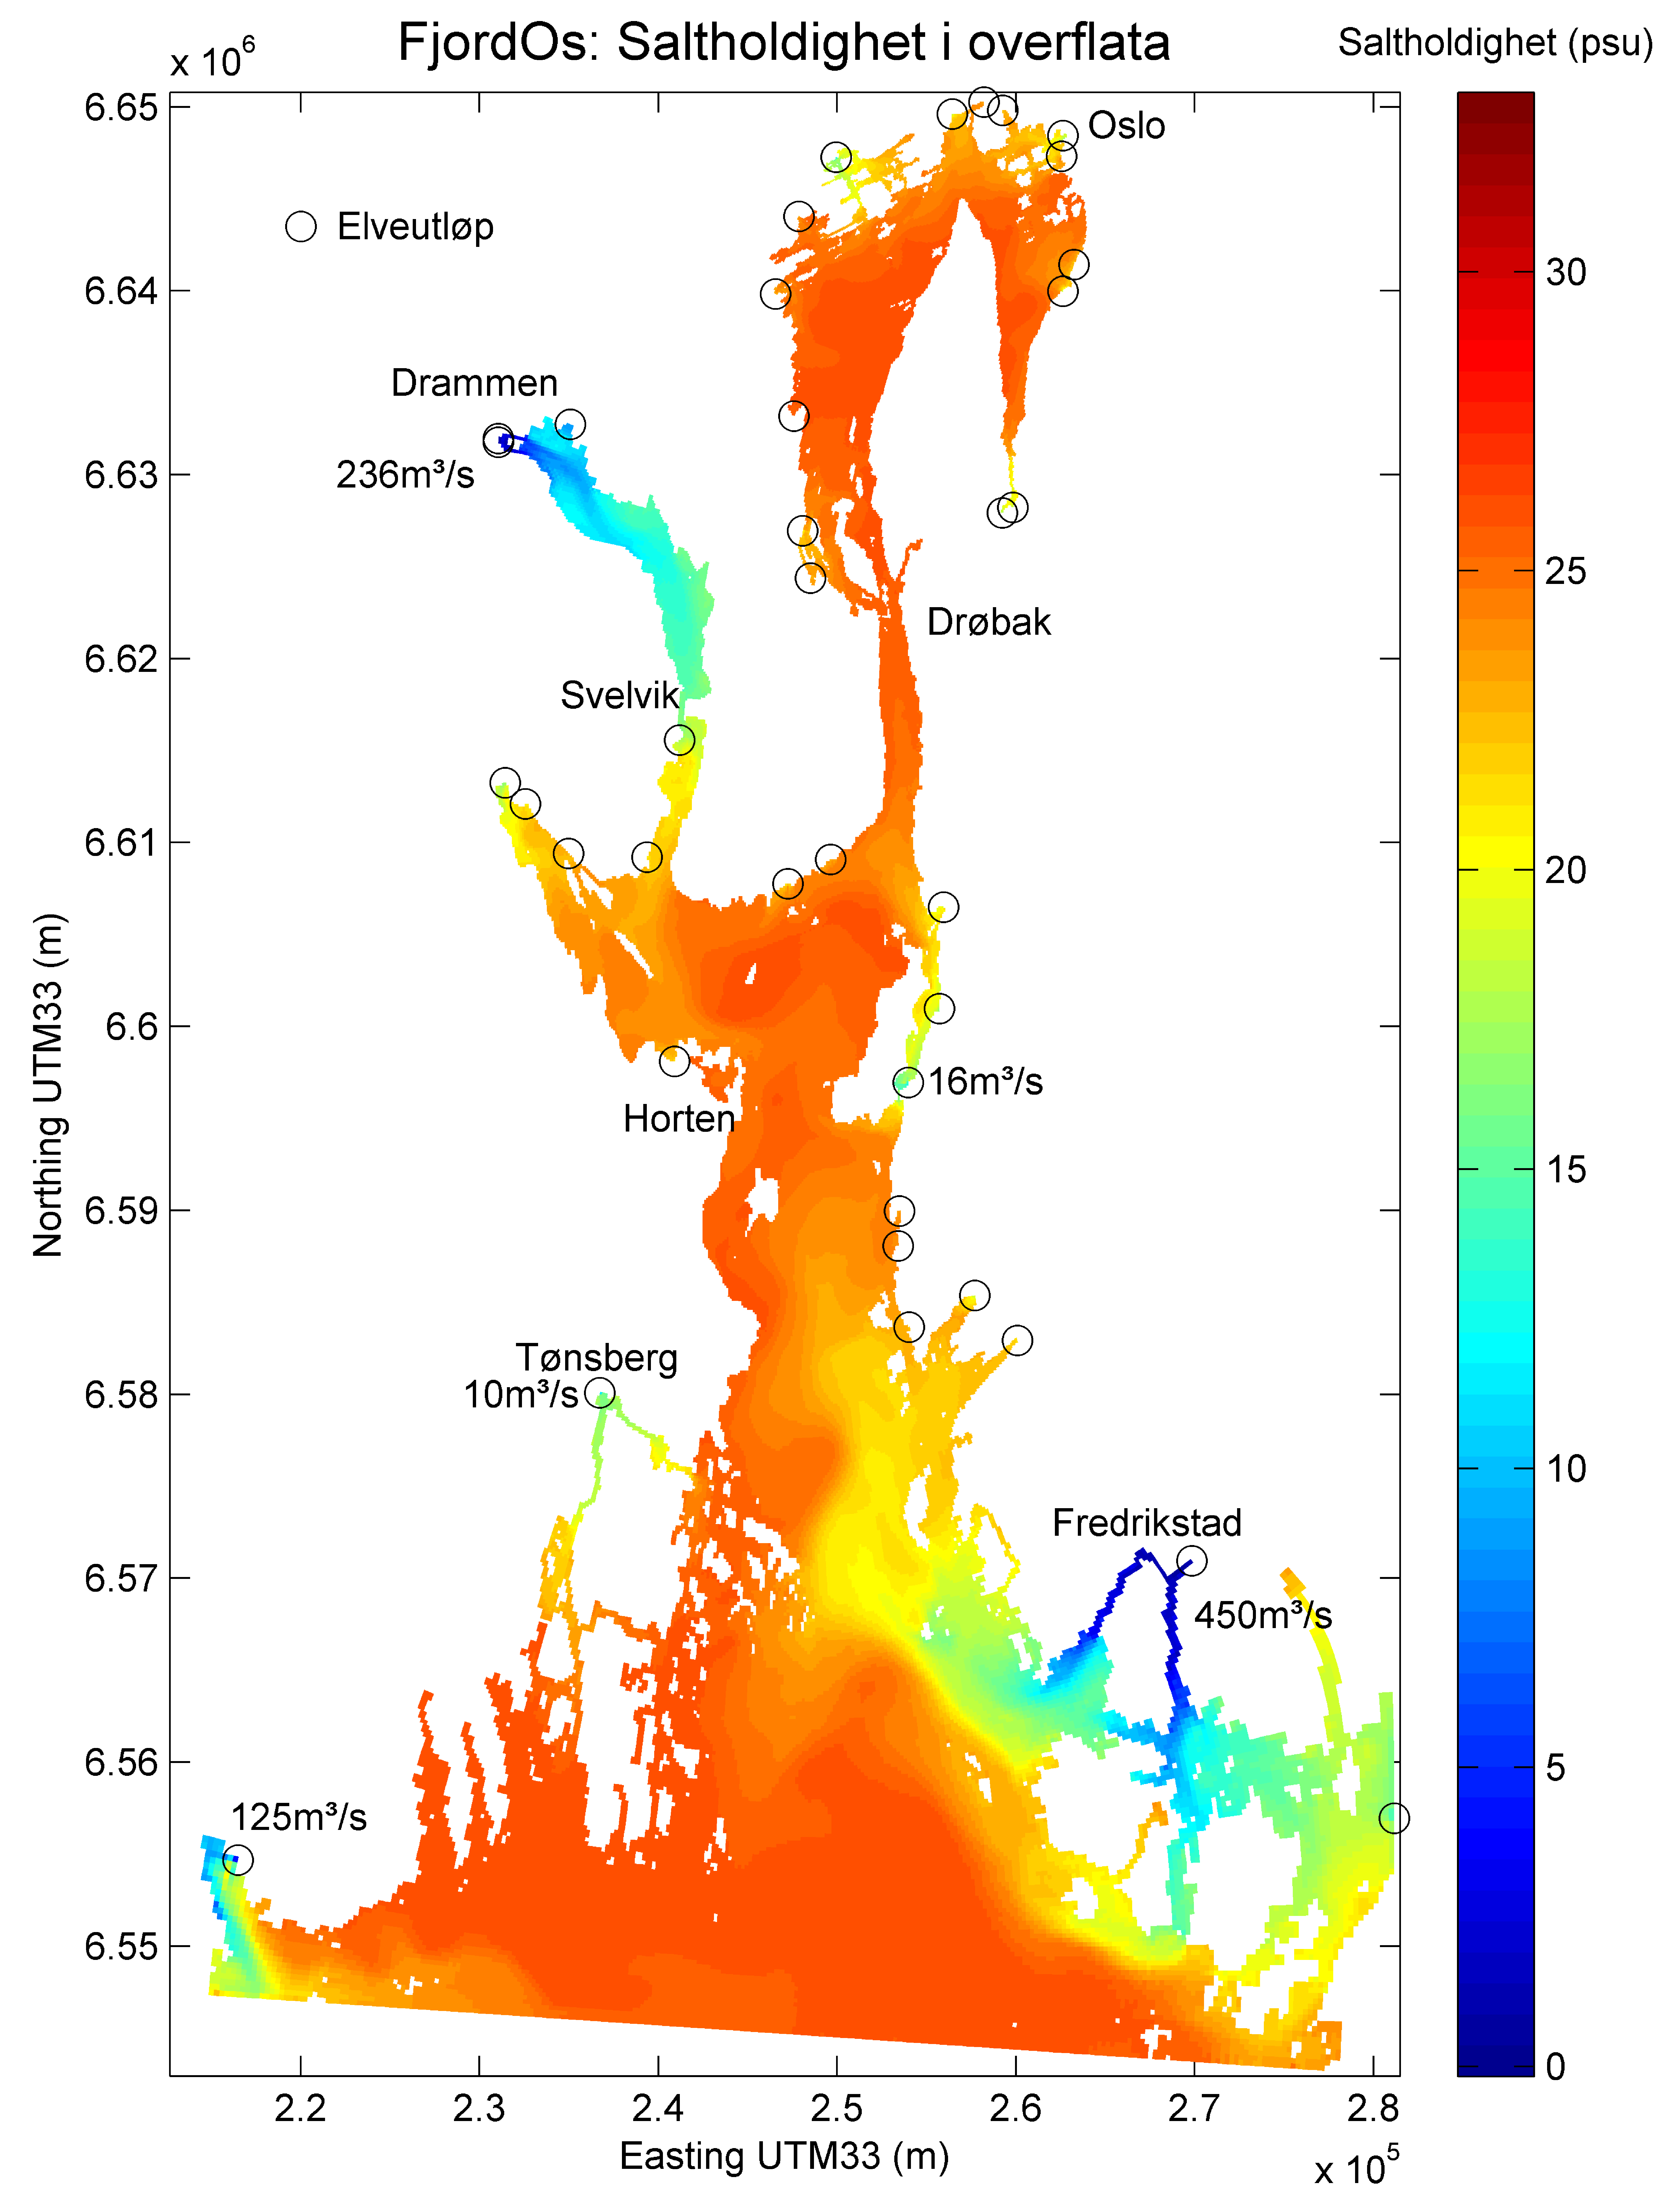
\includegraphics[height=9cm]{fjordos_rivers}}
  \end{pspicture}
% Figure caption is below the figure
  \caption{Left panel shows the many rivers (blue solid lines) emptying freshwater to the fjord (from NVE elvenett). The red numbers indicate a Main Catchment Area (MCA). The red dots indicate the location of the individual rivers discharging freshwater to Oslofjord (cf. Table \ref{tab:rivers01}). Some of the larger rivers, for instance Glomma, Drammenselva and Numedalsl{\aa}gen, are marked with a thicker blue line. Stations with water discharge measurements are shown with green dots and numbered with black numbers, e.g. q8. Right panel shows the location of the 37 rivers named in Table \ref{tab:rivers01}. }   
  \label{fig:rivers01}      
 \end{center}
\end{figure}
%

